\chapter{Background}
L'image Captioning richiede l'interazione tra i campi del \acrfull{nlp} e della \acrfull{cv}. In questo capitolo vengono presentati alcuni modelli, architetture e tecniche essenziali per comprendere il contenuto dei prossimi capitoli.
\section{Natural Language Processing}
Quando si lavora con il linguaggio naturale, il testo deve essere rappresentato in un formato leggibile dalla macchina prima di qualsiasi elaborazione, la qualità di qualsiasi compito successivo dipende fortemente dalla qualità della rappresentazione \cite{babic2020survey}.

I primi approcci per codificare il testo in un vettore, come il \acrfull{bow}, hanno diversi difetti: per esempio, i vettori sono solitamente sparsi \cite{chen2013alternative}.
I word embedding superano il problema della sparsità perché sono per definizione rappresentazioni vettoriali dense di lunghezza fissa per le parole. Tuttavia, hanno anche dimostrato di poter codificare informazioni sintattiche e semantiche \cite{almeida2019word}.
Vale la pena menzionare \acrfull{cbow}, \acrfull{sg}, che insieme sono spesso indicati come Word2Vec \cite{mikolov2013efficient}, e \acrfull{glove} \cite{pennington2014glove}; i quali sono tutti metodi che permettono di calcolare i vettori di word embedding; i primi due utilizzano reti neurali mentre l'ultimo utilizza statistiche di co-occorrenza globale.

Con la pubblicazione di Vaswani et al. \cite{vaswani2017attention}, nel 2017, i Transformer hanno iniziato a essere ampiamente impiegati nel campo del \acrshort{nlp}. 
Questa nuova architettura è basata su codificatori e decodificatori. I Transformer si basano su un'architettura sequence-to-sequence e sono stati originariamente utilizzati per la traduzione automatica. A differenza delle \acrfull{rnn}, che operano su sequenze e sono intrinsecamente sequenziali, i Transformer operano su set in modo parallelo. Invece di usare una singola codifica compressa proveniente dall'ultimo codificatore come nelle \acrshort{rnn}, nei Transformer i decodificatori possono accedere alle informazioni di ogni elemento in ingresso. Il nucleo di questi modelli è il meccanismo di self-attention che permette di cogliere le dipendenze nelle sequenze di input o output, rendendo il modello in grado di catturare informazioni contestuali e dipendenze più profonde, fornendo così una rappresentazione più significativa rispetto agli approcci precedenti. Siccome l'operazione di attenzione lavora su set e non su sequenze, il modello può essere limitato aggiungendo codifiche posizionali per trattare sequenze di testo.

\subsection{BERT}\label{bert_section}
Ispirandosi ai Transformer, Devlin et al. \cite{devlin2018bert} hanno presentato il modello \acrshort{bert} (\acrlong{bert}) nel 2019. A differenza dell'architettura originale dei Transformer, \acrshort{bert} non utilizza alcun decoder. Il fatto che utilizzi una pila di 12 codificatori bidirezionali dei Transformer rende \acrshort{bert} in grado di sfruttare sia il contesto sinistro che quello destro di ogni parola. Inoltre, grazie al meccanismo di attenzione ereditato dai Transformer, questa architettura può essere utilizzata per generare modelli linguistici molto potenti con una rappresentazione neurale densa.
Prima di alimentare il modello, il testo di input viene trasformato in una sequenza sotto forma di embedding tramite l'algoritmo WordPiece \cite{wu2016google}. Utilizzando questa rappresentazione, ogni parola è decomposta in sub-word comuni, permettendo così di migliorare la gestione delle parole rare. Il formato di una sequenza di input può contenere token speciali come \texttt{[CLS]} e \texttt{[SEP]}, dove il primo è il token di classificazione e il suo stato nascosto finale può essere usato come rappresentazione aggregata della sequenza per compiti di classificazione. Mentre il secondo identifica il token di separazione e può essere usato quando si devono differenziare le frasi che costituiscono l'input.

\begin{figure}[ht]
\centering
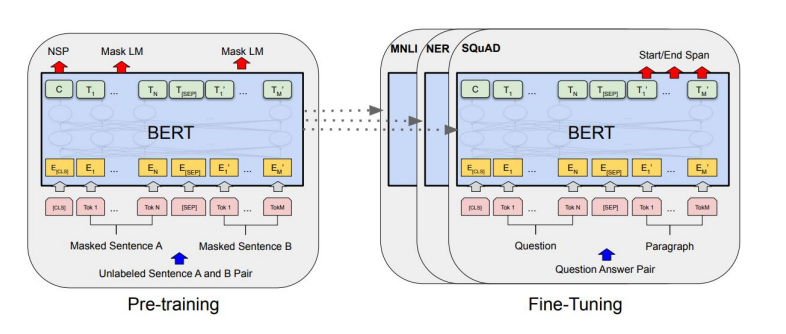
\includegraphics[width=0.9\textwidth]{bert}
\caption{Illustrazione riassuntiva del Pre-training e del Fine-Tuning di \acrshort{bert}. Source: Devlin et al. \cite{devlin2018bert}}\label{figura:bert}
\end{figure}

\acrshort{bert} ha guadagnato la maggior parte della sua popolarità grazie al fatto che può essere utilizzato in un'ampia varietà di compiti \acrshort{nlp} a valle senza grandi sforzi. Infatti, si presenta come un modello pre-addestrato su una grande quantità di dati e fornisce una rappresentazione generica del linguaggio che può essere messa a punto per affrontare qualsiasi problema (ad esempio, Question Answering, classificazione, Named-Entity Recognition, ecc.). La Figura \ref{figura:bert} mostra la procedura di pre-addestramento, la quale viene eseguita utilizzando due strategie:
\begin{enumerate}
    \item \textit{Masked Language Model}: per ogni sequenza di input, il 15\% dei token sono sostituiti dal token \texttt{[MASK]}. Successivamente, il modello viene addestrato per prevedere i valori originali dei token mascherati sfruttando il contesto sinistro e destro.
    \item \textit{Next Sentence Prediction (NSP)}: ogni sequenza di input è divisa in due parti separate dal token \texttt{[SEP]}. Poi, il 50\% delle sequenze viene modificato sostituendo la seconda parte con una casuale da un'altra sequenza. Infine, il modello è addestrato a distinguere sequenze positive e negative.
\end{enumerate}
L'alta qualità della rappresentazione del testo è ottenuta a spese di un elevato costo computazionale. Il modello \acrshort{bert} è originariamente disponibile in due versioni: \acrshort{bert} base (110M parametri) e \acrshort{bert} large (340M parametri). Queste dimensioni del modello richiedono elevate capacità di memoria e rendono la procedura di addestramento non accessibile a tutti. 
Per questo motivo, sono state proposte e rese disponibili diverse nuove versioni.

\section{Computer Vision}
Quando si lavora con le immagini, esse devono essere rappresentate in un formato comprensibile dalla macchina prima di qualsiasi elaborazione, la qualità delle caption finali dipende fortemente dalla qualità della rappresentazione dell'immagine.
\subsection{Object Detection}
Molti approcci di Image Captioning che hanno consentito il raggiungimento di risultati allo stato dell'arte hanno sfruttato l'Object Detection per effettuare la comprensione e l'estrazione delle feature delle immagini.

L'Object Detection è una tecnica di \acrlong{cv} che identifica e localizza degli oggetti all'interno di un'immagine. In particolare, il rilevamento degli oggetti viene effettuato tramite dei riquadri di delimitazione (bounding box) attorno agli oggetti rilevati e a ognuno di essi viene assegnata una classe (tag) che identifica l'oggetto identificato. La bounding box è di forma rettangolare e descrive la posizione spaziale di un oggetto tramite un vettore, il quale è composto dalle coordinate x e y dell'angolo superiore sinistro del rettangolo e da quelle dell'angolo inferiore destro.
Quando si usano i modelli di Object Detection la rappresentazione finale dell'immagine viene ottenuta tramite le rappresentazioni vettoriali dei vari oggetti che la compongono, solitamente queste feature vengono estratte da un layer intermedio del modello di detection.

\subsubsection{Faster R-CNN}\label{faster_rcnn_model}
Il modello di Object Detection più utilizzato è \acrshort{faster_rcnn} \cite{ren2015faster} (Figura \ref{figura:faster_rcnn}), il quale è una variante di \acrshort{rcnn} \cite{girshick2014rich} e di \acrshort{fast_rcnn} \cite{girshick2015fast}.
\acrshort{faster_rcnn} è stato progettato per identificare istanze di oggetti appartenenti a certe classi e per localizzarle tramite bounding box.
\begin{figure}[ht]
\centering
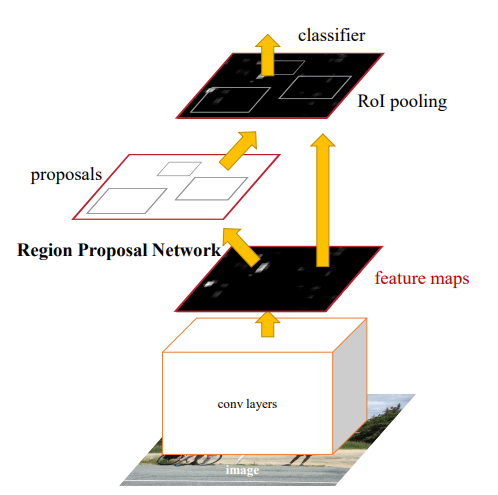
\includegraphics[width=0.5\textwidth]{faster_rcnn}
\caption{Illustrazione raffigurante l'architettura di \acrshort{faster_rcnn}. Source: Ren et al. \cite{ren2015faster}}\label{figura:faster_rcnn}
\end{figure}

Questo modello rileva gli oggetti tramite due fasi:
\begin{enumerate}
    \item \acrfull{rpn}: riceve come input un'immagine (di qualsiasi dimensione) e produce un insieme di proposte di oggetti. Questa componente è implementata tramite una piccola rete che viene fatta scorrere sulle feature estratte da un layer intermedio di una \acrshort{cnn} chiamata backbone. In ogni posizione spaziale la rete predice: un punteggio di objectness indipendente dalla classe e un raffinamento della bounding box chiamato anchor box, quest'ultimo ha una scala e una proporzione specifica. Con più anchor box di riferimento esistono più scale e proporzioni per la singola regione. Quindi, ciascuna regione viene mappata su ciascuna anchor box di riferimento, rilevando così oggetti a scale e proporzioni diverse. Usando la soppressione greedy non massima con una soglia di \acrfull{iou} vengono selezionate le proposte di regioni, le quali servono come input per la seconda fase;
    \item \acrfull{roipool}: usa il max pooling per convertire le feature all'interno di una qualsiasi regione di interesse in una piccola mappa di feature (viene effettuato un processo di quantizzazione sulle \acrshort{roi} ottenendo una granularità discreta delle mappe delle feature).
\end{enumerate}
Infine, i vettori di feature estratti utilizzando il \acrlong{roipool} vengono passati ad alcuni Fully Connected layer, l'ultimo di questi layer è suddiviso in due rami dove uno determina le classi e l'altro le bounding box degli oggetti rilevati.


Nonostante il modello \acrshort{faster_rcnn} non sia recente ed esistano modelli di Object Detection con performance superiori, risulta molto utilizzato nell'Image Captioning perché può essere utilizzato con backbone pre-addestrate sul dataset ImageNet (per esempio \acrshort{resnet} risulta essere la più popolare) e perché si basa sui layer convoluzionali, queste due caratteristiche permettono l'ottenimento di un migliore bias induttivo per la codifica delle informazioni visive delle regioni \cite{jiang2020defense}.

\subsection{Image Segmentation}
L'Image Segmentation oltre a predire la bounding box e l'etichetta di classe per ogni oggetto rileva anche la maschera di segmentazione, la quale permette di estrarre solo l'oggetto rilevato dall'immagine senza includere i pixel superflui dello sfondo.

Esistono tre tipologie principali di segmentazione:
\begin{enumerate}
\item \textbf{Semantic Segmentation}: assegna un'etichetta di classe a ogni pixel di un'immagine;
\item \textbf{Instance Segmentation}: rileva e delinea ogni istanza di oggetto con una maschera di segmentazione;
\item \textbf{Panoptic Segmentation} \cite{kirillov2019panoptic}: tratta sia le classi di tipo \textit{stuff} sia di tipo \textit{thing}, unificando i due tipi di segmentazione esposti precedentemente. 
Con stuff ci si riferisce a regioni amorfe e non numerabili di texture o materiale simile individuabili tramite la Semantic Segmentation (per esempio: sky, ground, grass, etc), mentre con thing ci si riferisce a oggetti numerabili individuabili tramite Instance Segmentation (per esempio people, animal, tool, etc).
L'attività di Panoptic Segmentation prevede l'assegnazione di un'etichetta semantica e di un ID di istanza per ciascun pixel di un'immagine, richiedendo la generazione di segmentazioni di scena dense, coerenti e complete.
\end{enumerate}
\begin{figure}[ht]
\centering
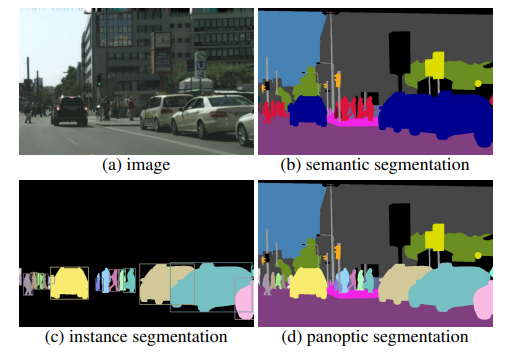
\includegraphics[width=0.8\textwidth]{segmentazioni}
\caption{Illustrazione in cui si può vedere la differenza di risultati tra le tipologie di Image Segmentation. Source: Kirillov et al. \cite{kirillov2019panoptic}}
\end{figure}
\newpage
\subsubsection{Mask R-CNN} \label{mask_section}
Un modello molto popolare di Instance Segmentation è \acrshort{mask_rcnn} \cite{he2017mask} (Figura \ref{mask_img}), il quale risulta molto interessate perché può essere visto come il miglioramento del modello di Object Detection \acrshort{faster_rcnn} (il quale si comporta bene nel contesto dell'Image Captioning, vedere sezione \ref{faster_rcnn_model}) con un ramo aggiuntivo che si occupa della predizione della maschera, questo ramo è una piccola \acrfull{fcn}.
\begin{figure}[ht]
\centering
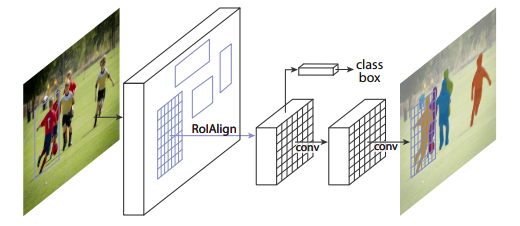
\includegraphics[width=0.8\textwidth]{mask_rcnn}
\caption{Illustrazione raffigurante l'architettura di \acrshort{mask_rcnn}. Source: He et al. \cite{he2017mask}}\label{mask_img}
\end{figure}


L'unica differenza tra i due modelli è la rimozione delle quantizzazioni utilizzate nel \acrshort{roipool}, le quali introducono disallineamenti tra le \acrshort{roi} e le feature estratte generando errori nella previsione di maschere accurate al pixel. Gli autori per risolvere questo problema hanno proposto un livello RoIAlign che rimuove la quantizzazione di \acrshort{roipool}, allineando correttamente le feature estratte con l'input, e usano l'interpolazione bilineare \cite{jaderberg2015spatial}, per calcolare i valori esatti delle feature di input in quattro posizioni regolarmente campionate in ogni bin \acrshort{roi} e aggregano il risultato (usando max o media).


\subsubsection{DETR} \label{detr_section}
\acrshort{detr} (\acrlong{detr}) \cite{carion2020end} è un modello di Object Detection che ha riscontrato successo nel task di Panoptic Segmentation. Questo modello è basato su Transformer e sulla bipartite matching loss per la previsione diretta del set.
\begin{figure}[ht]
\centering
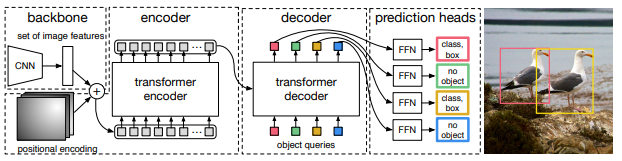
\includegraphics[width=0.85\textwidth]{detr}
\caption{Illustrazione raffigurante l'architettura di \acrshort{detr} per il task di Object Detection. Source: Carion et al. \cite{carion2020end}}\label{detr_img}
\end{figure}



L'architettura di DETR contiene tre componenti:
\begin{enumerate}
    \item Backbone \acrshort{cnn}: utilizzata per estrarre una rappresentazione compatta delle feature dell'immagine di input;
    \item Encoder-Decoder Transformer: 
    \begin{itemize}
        \item Transformer Encoder: riceve come input la rappresentazione precedentemente calcolata e genera delle codifiche più significative dell'immagine di input, contenenti informazioni posizionali.
        L'Encoder è composto da un modulo di multi-head self-attention e da una \acrfull{ffn}, inoltre agli input di ogni attention layer viene aggiunta una codifica posizionale (perché l'architettura del Transformer è invariante alle permutazioni);
        \item Transformer Decoder: riceve come input la memoria dell'Encoder e N object queries (sono le codifiche posizionali apprese). Trasforma gli N embedding di dimensione d usando il meccanismo multi-headed self- and encoder-decoder attention sfruttando la codifica ricevuta, questo si differenzia da quello standard perché permette la decodifica degli N oggetti in parallelo a ogni strato del decoder. Infine, gli embedding ottenuti, rappresentanti N codifiche di oggetti, vengono forniti come input alla rete \acrshort{ffn};
    \end{itemize}
    \item \acrfull{ffn}: riceve le N proposte ed effettua le predizioni finali del rilevamento.
\end{enumerate}

\acrshort{detr} ha avuto successo nella Panoptic Segmentation poiché può essere naturalmente esteso aggiungendo una mask head in cima agli output del decoder, riesce a trattare le classi stuff e thing in modo unificato.

